% !TeX root = ../main.tex

\documentclass[../main.tex]{subfiles}
\begin{document}

\section{Kết quả thực nghiệm và đánh giá hiệu năng hệ thống}
\label{sec:experimental_results}

Chương này trình bày kết quả thực nghiệm của hệ thống giám sát tháp giải nhiệt IoT được triển khai trong điều kiện thực tế. Nghiên cứu bao gồm phân tích dữ liệu thu thập trong khoảng thời gian 10 ngày liên tục, đánh giá hiệu năng các thành phần hệ thống và xác thực tính hiệu quả của giải pháp đề xuất. Thí nghiệm được thực hiện tại phòng thí nghiệm với mô hình tháp giải nhiệt thu nhỏ, trong điều kiện môi trường được kiểm soát để đảm bảo tính khách quan và khả năng tái lập của kết quả.

Phân tích thống kê dữ liệu thực nghiệm cho thấy xu hướng suy giảm hiệu suất rõ rệt theo thời gian và sự tương quan mạnh với các điều kiện môi trường. Kết quả này khẳng định độ tin cậy của hệ thống cảm biến và khả năng phát hiện các biến đổi tinh tế trong hiệu suất vận hành.

\section{Thiết lập thí nghiệm}
\label{sec:experimental_setup}

\subsection{Môi trường thí nghiệm}
\label{sec:test_environment}

Thí nghiệm được thực hiện tại phòng thí nghiệm Nghiên cứu Nhiên liệu và Năng lượng sạch (FCE Lab) trong điều kiện môi trường kiểm soát nhằm đảm bảo độ tin cậy của kết quả. Mô hình tháp giải nhiệt thu nhỏ được sử dụng để giải nhiệt cho tải nhiệt. Tải nhiệt đầu vào được duy trì ổn định bằng rơ-le bán dẫn (SSR) suốt quá trình khảo sát. Việc kiểm soát tải nhiệt này giúp đảm bảo tính nhất quán của các phép đo và tăng độ chính xác trong đánh giá hiệu suất hệ thống.

\begin{figure}
    \centering
    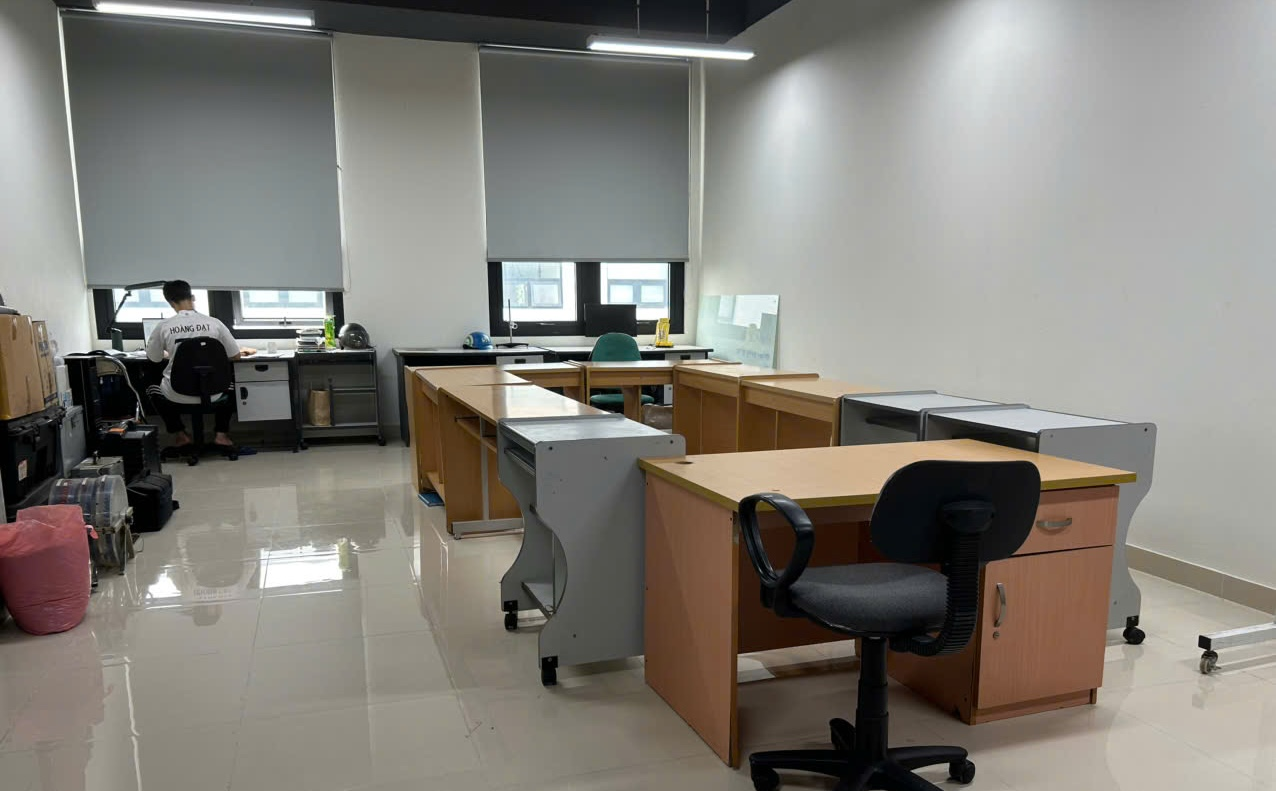
\includegraphics[width=1\textwidth]{Hinhve/fcelab.jpg}
    \caption{Phòng thí nghiệm Nghiên cứu Nhiên liệu và Năng lượng sạch - FCE Lab, Đại học Bách khoa Hà Nội}
    \label{fig:fcelab}
\end{figure}

Môi trường phòng thí nghiệm được điều chỉnh bởi hệ thống điều hòa không khí, tạo ra các điều kiện nhiệt độ và độ ẩm biến thiên theo chu kỳ. Cách thức vận hành này cho phép mô phỏng đặc tính môi trường công nghiệp thực tế. Hệ thống điều hòa không khí được vận hành theo lịch trình cố định với nhiệt độ cài đặt $26{^\circ\mathrm{C}} \pm 1{^\circ\mathrm{C}}$. Hệ thống này hoạt động chủ yếu trong khung giờ làm việc (8:00-17:00) khi có sự hiện diện của con người và thiết bị điện tử phát nhiệt. Ngoài khung giờ này, hệ thống điều hòa ngừng hoạt động, cho phép nhiệt độ và độ ẩm biến thiên tự nhiên.

Mô hình vận hành này tạo điều kiện đánh giá khả năng thích ứng của hệ thống giám sát trong các chế độ làm việc khác nhau. Đồng thời, thiết lập này cho phép xác thực độ chính xác của các phép tính hiệu suất dưới tác động của các yếu tố môi trường biến đổi.

\subsection{Cấu hình hệ thống đo lường và lắp đặt cảm biến}
\label{sec:measurement_system_config}

Các cảm biến được bố trí theo cấu hình tiêu chuẩn nhằm đảm bảo tính đại diện và giảm thiểu sai lệch do điều kiện biên. Đầu đo nhiệt độ nước vào (\textbf{DS18B20-01}) được đặt trên tuyến ống cấp nước nóng, cách cửa vào tháp khoảng $0{,}3$ m để bảo đảm dòng chảy ổn định trước điểm đo. Tương tự, đầu đo nhiệt độ nước ra (\textbf{DS18B20-02}) được lắp trên tuyến ống nước lạnh ngay sau cửa ra tháp, nhằm hạn chế tối đa ảnh hưởng của trao đổi nhiệt với môi trường xung quanh.

Cảm biến lưu lượng \textbf{YF-S201} được lắp trên tuyến ống tuần hoàn chính, bố trí sau bơm và trước tải nhiệt. Tại vị trí này, đường ống được bố trí nằm trên một mặt phẳng ngang nhằm đảm bảo yêu cầu kỹ thuật của nhà sản xuất \cite{datasheet_YFS201}. Cấu hình lắp đặt này cũng nhằm giảm tiếp xúc trực tiếp với vùng nước có nhiệt độ quá cao và hạn chế tác động của bọt khí hoặc chất rắn lơ lửng. Những yếu tố này có thể ảnh hưởng đến đáp ứng cơ học của turbine trong cảm biến.

Đối với môi trường không khí, cảm biến \textbf{DHT22} được đặt tại vị trí đại diện quanh tháp, tránh bức xạ mặt trời trực tiếp và các nguồn nhiệt cục bộ. Khi cần thiết, hệ thống sử dụng che chắn bức xạ (radiation shield) để bảo đảm số đo phản ánh điều kiện khí quyển tại chỗ.

\begin{figure}[H]
    \centering
    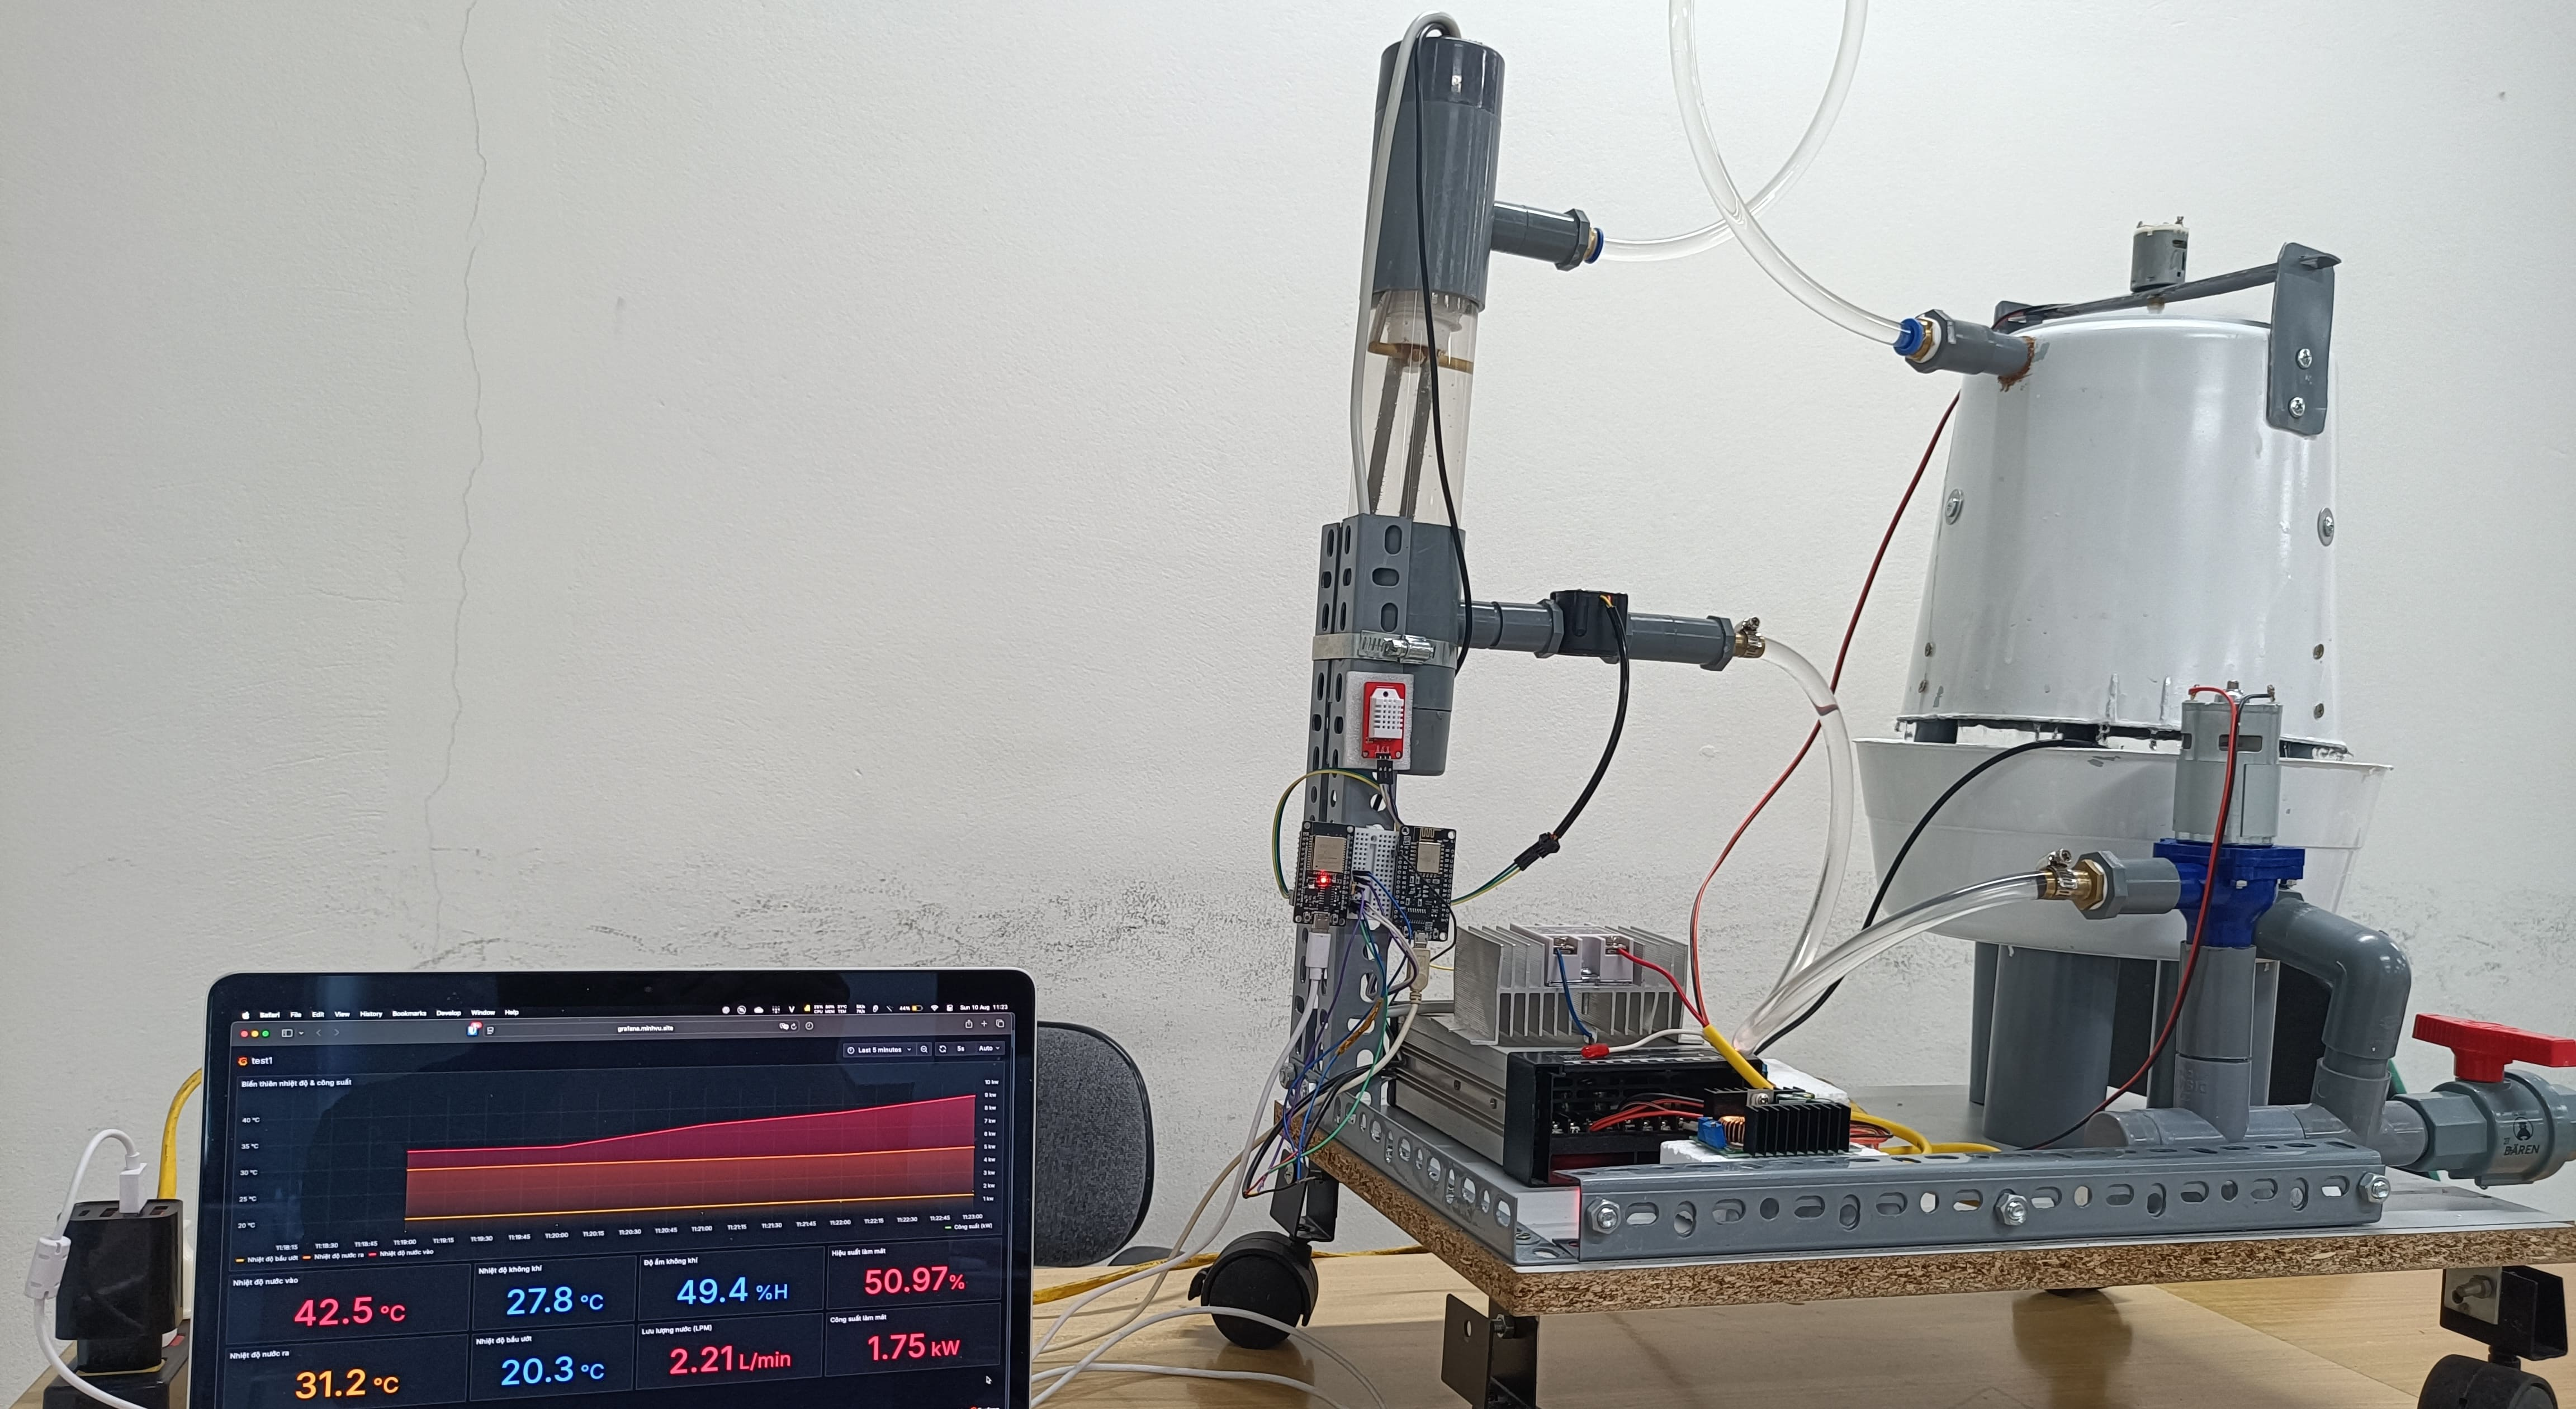
\includegraphics[width=1\textwidth]{Hinhve/lap_dat.jpg}
    \caption{Hoàn thành cấu hình và lắp đặt cảm biến cho hệ thống, mô hình đã hoạt động và gửi dữ liệu vận hành về máy chủ.}
    \label{fig:lap_dat}
\end{figure}

Trong phạm vi thí nghiệm này, hệ thống \emph{không} tiến hành hiệu chuẩn ngoại (traceable calibration). Các đánh giá độ chính xác dựa trên đặc tính danh định do nhà sản xuất công bố. Cụ thể, \textbf{DS18B20} có sai số điển hình $\pm 0{,}5^\circ\mathrm{C}$ trong khoảng $-10^\circ\mathrm{C}$ đến $+85^\circ\mathrm{C}$. \textbf{DHT22} đạt sai số nhiệt độ khoảng $\pm 0{,}5^\circ\mathrm{C}$ và sai số độ ẩm điển hình $\pm 2\%$RH (tối đa $\pm 5\%$RH) trong dải 0–100\%RH. Cảm biến lưu lượng \textbf{YF-S201} có sai số điển hình khoảng $\pm 10\%$ lưu lượng danh định \cite{datasheet_DS18B20,datasheet_DHT22,datasheet_YFS201}.

Các giá trị này được sử dụng làm giới hạn bất định đo trong phân tích kết quả. Trong tương lai, để cải thiện độ tin cậy tuyệt đối của các đại lượng suy diễn (ví dụ: công suất giải nhiệt), nghiên cứu khuyến nghị hiệu chuẩn hiện trường cho \textbf{YF-S201} theo phương pháp thể tích–thời gian và kiểm định chéo nhiệt độ bằng cặp đầu đo tham chiếu.

\subsection{Thông số vận hành}
\label{sec:operating_parameters_config}

Thí nghiệm được thực hiện liên tục trong 10 ngày (240 giờ), từ 07{:}00 ngày 08/08/2025 đến 07{:}00 ngày 18/08/2025 (UTC+7)\footnote{Ghi chú về mốc thời gian: cách viết "từ ngày 08/08/2025 đến ngày 18/08/2025" có thể gây hiểu nhầm về tính "bao gồm" ngày cuối; trong báo cáo này, khoảng thời gian được hiểu là \emph{bắt đầu} tại 08/08/2025 07{:}00 và \emph{kết thúc} tại 18/08/2025 07{:}00, tương ứng 240 giờ.}. Dữ liệu được lấy mẫu với chu kỳ $30$ s, tương đương $120$ mẫu/giờ, nhằm bảo đảm độ phân giải thời gian đủ để quan sát các biến thiên nhanh của hệ thống.

Với khung thời gian và tần suất lấy mẫu này, tổng số điểm dữ liệu lý thuyết là $28.800$ mẫu. Trong thực tế, hệ thống thu thập được $28.720$ mẫu cho 9 thông số đo lường, tương ứng tỷ lệ thành công $99{,}72\%$ $(28.720/28.800)$. Các thông số được theo dõi bao gồm nhiệt độ nước vào, nhiệt độ nước ra, nhiệt độ không khí, độ ẩm không khí, lưu lượng nước tuần hoàn, hiệu suất làm mát và nhiệt độ bầu ướt.

Trong toàn bộ giai đoạn thí nghiệm, hệ thống vận hành tại các thiết lập danh định nhằm đánh giá ảnh hưởng của biến thiên môi trường và quá trình lão hóa tự nhiên của hệ thống. Lưu lượng nước tuần hoàn được duy trì ổn định ở mức \(1{,}91 \pm 0{,}05\) L/min. Quạt làm mát chạy ở công suất định mức. Tải nhiệt được điều khiển bằng rơ-le bán dẫn (SSR) với việc điều chỉnh duty cycle để duy trì điều kiện vận hành ổn định. Do hiệu suất tháp giải nhiệt có xu hướng suy giảm theo thời gian, duty cycle của SSR được giảm dần từ 30\% trong những ngày đầu xuống còn 19\% vào cuối thí nghiệm nhằm bảo đảm nhiệt độ nước vào không vượt quá giới hạn thiết kế.

Nhiệt độ nước vào tháp được quan sát trong khoảng \(33{,}4^\circ\mathrm{C}\) đến \(35{,}1^\circ\mathrm{C}\) với giá trị trung bình \(34{,}2^\circ\mathrm{C} \pm 0{,}4^\circ\mathrm{C}\). Nhiệt độ không khí xung quanh tháp được duy trì trong khoảng \(27{,}7^\circ\mathrm{C}\) đến \(29{,}4^\circ\mathrm{C}\) với giá trị trung bình \(28{,}5^\circ\mathrm{C} \pm 0{,}4^\circ\mathrm{C}\). Độ ẩm tương đối không khí dao động từ 71{,}0\% đến 87{,}4\%, với giá trị trung bình 79{,}1\% \(\pm 4{,}2\%\).

Để mô phỏng điều kiện vận hành thực tế của hệ thống công nghiệp, nước tuần hoàn được điều chỉnh thành phần theo kế hoạch định sẵn với việc bổ sung tạp chất hòa tan và chất rắn lơ lửng. Quá trình này nhằm tái tạo đặc tính nước công nghiệp điển hình và thúc đẩy hình thành cặn bẩn trên bề mặt trao đổi nhiệt trong khoảng thời gian thí nghiệm hạn chế.

Phương pháp điều chỉnh thành phần nước cho phép quan sát quá trình suy giảm hiệu suất nhiệt do tích tụ khoáng chất và bám bẩn vật lý mà không bị ảnh hưởng bởi các biến số môi trường khác. Sự gia tăng dần độ cứng nước và hàm lượng chất lơ lửng tạo điều kiện mô phỏng quá trình lão hóa tự nhiên của hệ thống. Điều này cho phép đánh giá xu hướng biến đổi hiệu suất trong điều kiện gần với thực tế vận hành công nghiệp.

\section{Kết quả thu thập dữ liệu}
\label{sec:data_collection_results}

\subsection{Dữ liệu nhiệt độ và lưu lượng}
\label{sec:temperature_flow_data}

\begin{figure}[H]
    \centering
    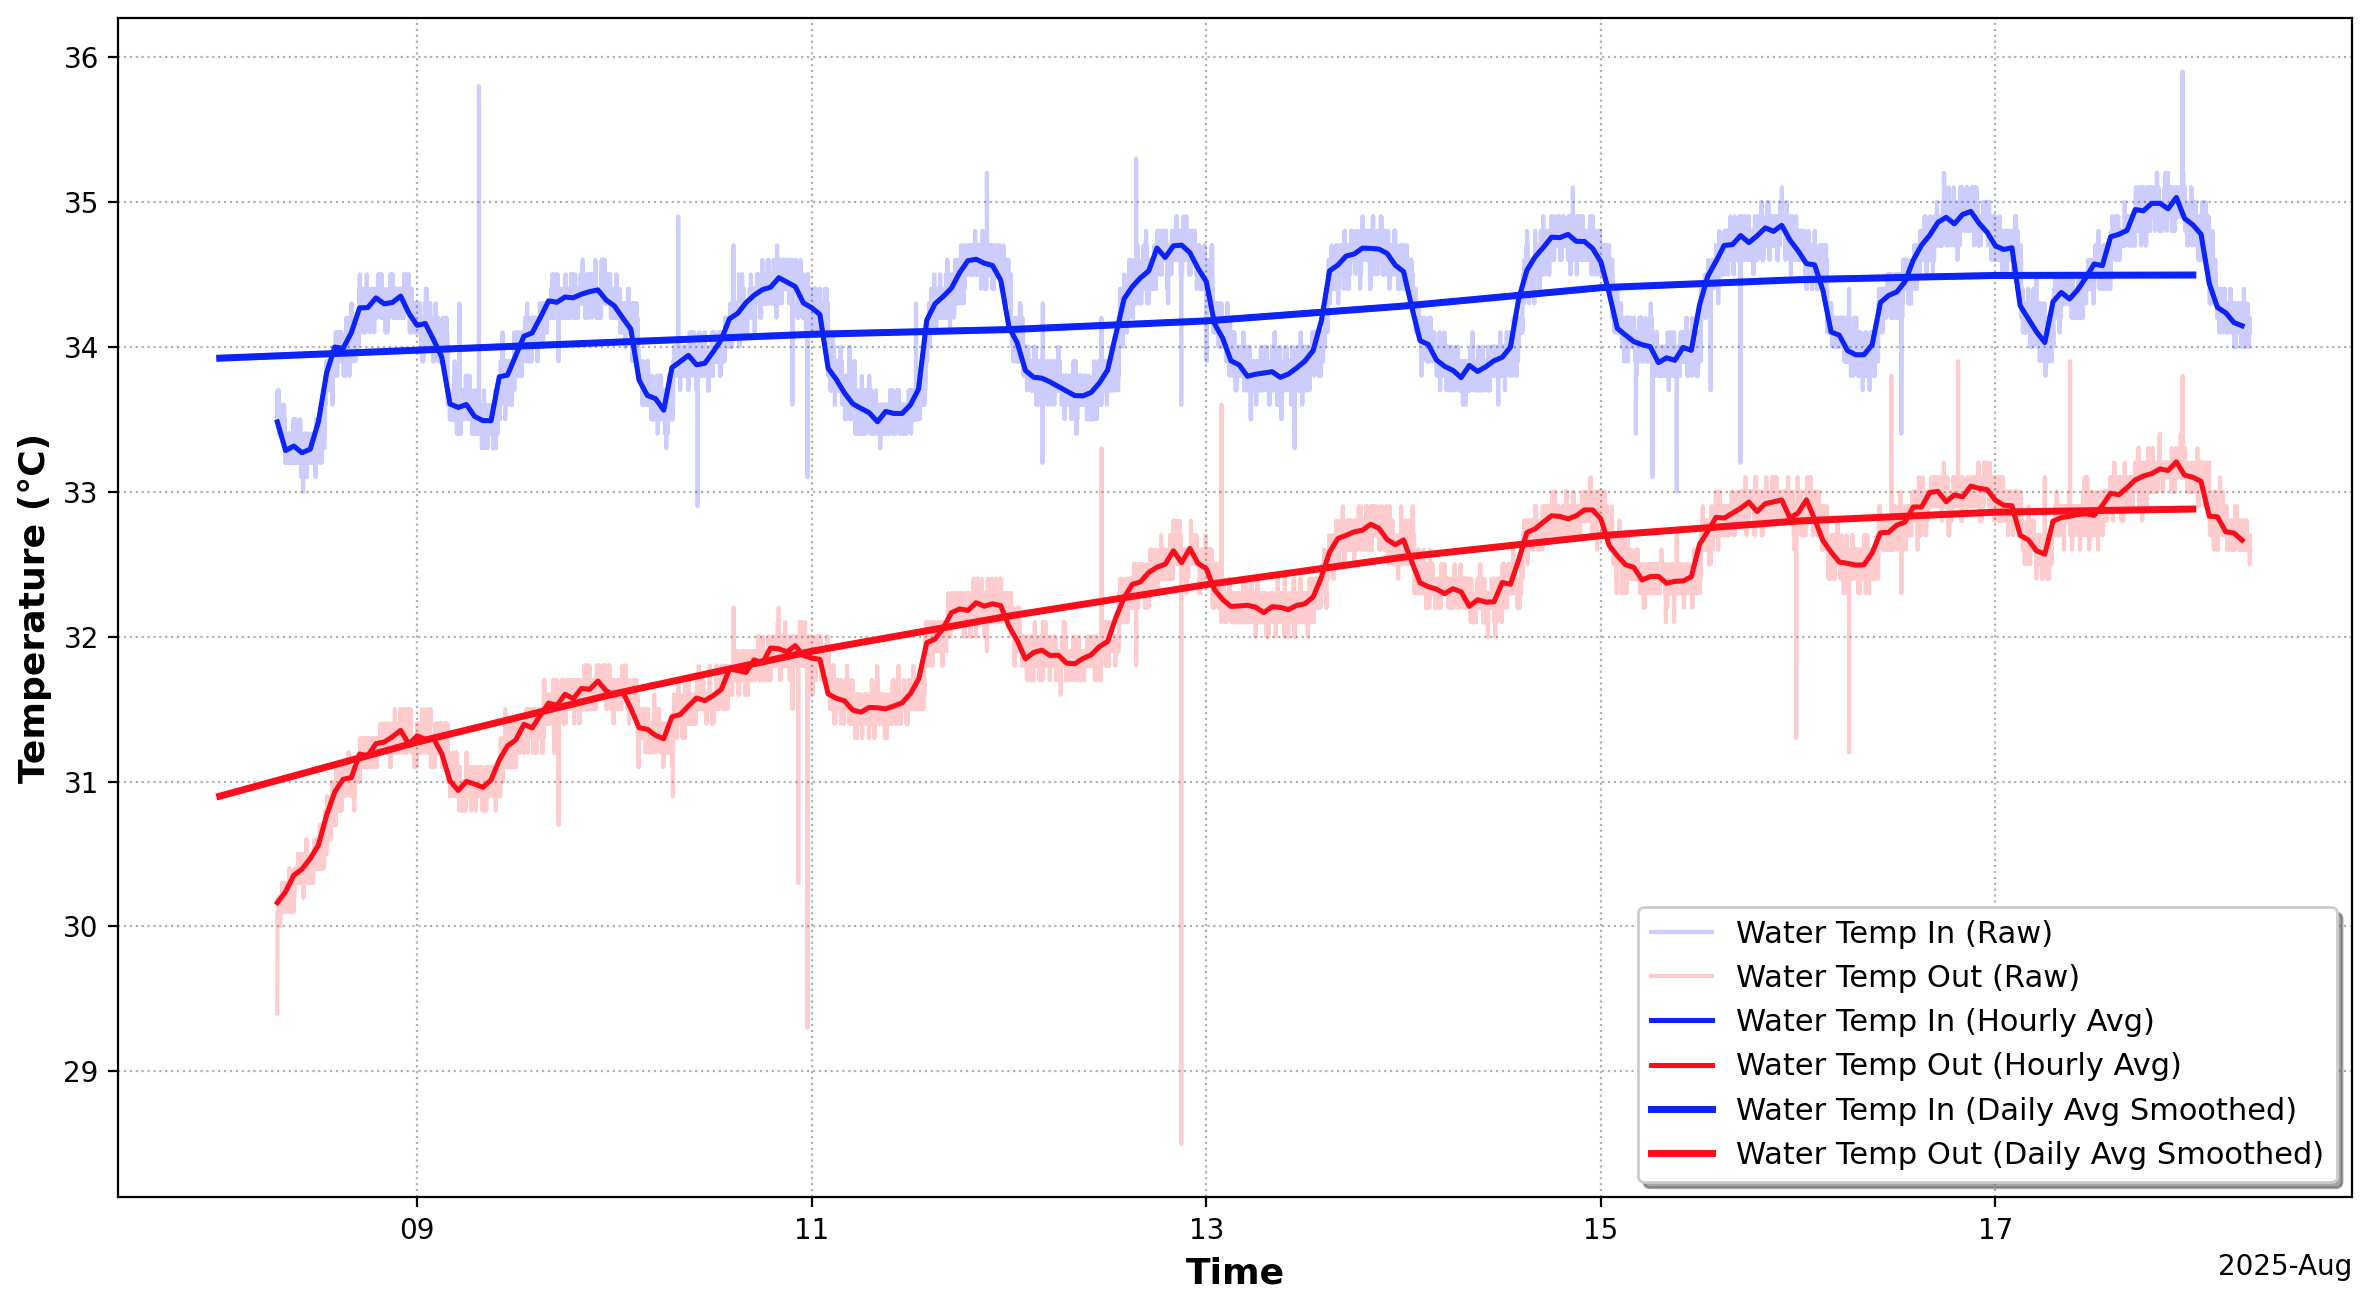
\includegraphics[width=1\textwidth]{../Hinhve/nhiet_do_nuoc.png}
    \caption{Biểu đồ nhiệt độ nước vào/ra theo thời gian}
    \label{fig:water_temperature_chart}
\end{figure}

Kết quả thu thập dữ liệu trong 10 ngày thí nghiệm cho thấy sự biến đổi rõ rệt của các thông số vận hành theo chu kỳ ngày-đêm. Những biến đổi này phản ánh ảnh hưởng mạnh mẽ của điều kiện môi trường đến hiệu suất tháp giải nhiệt. Nhiệt độ nước vào tháp giải nhiệt dao động từ $33{,}4{^\circ\mathrm{C}}$ đến $35{,}1{^\circ\mathrm{C}}$, với giá trị trung bình $34{,}2{^\circ\mathrm{C}} \pm 0{,}4{^\circ\mathrm{C}}$.

Phân tích tương quan Pearson cho thấy nhiệt độ không khí xung quanh (dao động từ $27{,}7{^\circ\mathrm{C}}$ đến $29{,}4{^\circ\mathrm{C}}$) có hệ số tương quan r = -0,285 với hiệu suất làm mát. Trong khi đó, độ ẩm tương đối (biến thiên trong khoảng 71{,}0\% đến 87{,}4\%) thể hiện tương quan nghịch mạnh với hệ số r = -0,842. Đặc biệt, hiệu suất tháp giải nhiệt bị ảnh hưởng rõ rệt bởi độ ẩm không khí. Điều này cho thấy tầm quan trọng của việc kiểm soát điều kiện môi trường trong vận hành hệ thống trao đổi nhiệt.

Nhiệt độ nước ra từ tháp giải nhiệt biến đổi từ $31{,}2{^\circ\mathrm{C}}$ đến $33{,}5{^\circ\mathrm{C}}$, với giá trị trung bình $32{,}2{^\circ\mathrm{C}} \pm 0{,}7{^\circ\mathrm{C}}$. Chênh lệch nhiệt độ trung bình ($\Delta T$) đạt $2{,}1{^\circ\mathrm{C}} \pm 0{,}5{^\circ\mathrm{C}}$, cho thấy hiệu quả làm mát vừa phải của hệ thống trong suốt thời gian thí nghiệm. Phân tích xu hướng dài hạn cho thấy $\Delta T$ duy trì tương đối ổn định nhưng có xu hướng giảm theo thời gian. Xu hướng này phản ánh sự suy giảm hiệu suất của hệ thống trong điều kiện tải ổn định và môi trường độ ẩm cao.

Lưu lượng nước tuần hoàn được duy trì ổn định cao ở mức $1{,}91 \pm 0{,}05$ L/min trong suốt thời gian thí nghiệm. Kết quả này chứng tỏ độ tin cậy cao của hệ thống bơm và cảm biến đo lường. Hệ số biến thiên chỉ 2{,}6\% cho thấy hệ thống hoạt động rất ổn định với sự biến động tối thiểu. Hiệu suất làm mát trung bình đạt $26{,}0 \pm 4{,}6\%$, thấp hơn mong đợi do điều kiện môi trường có độ ẩm cao. Điều kiện này ảnh hưởng đáng kể đến quá trình bay hơi và trao đổi nhiệt.

\begin{table}[H]
\centering
\renewcommand{\arraystretch}{1.3}
\caption{Thống kê thông số vận hành theo khung giờ trong ngày}
\label{tab:temperature_statistics}
\resizebox{\textwidth}{!}{
\begin{tabular}{|l|c|c|c|c|}
\hline
\textbf{Khung giờ} & \textbf{T\textsubscript{in}/T\textsubscript{out} ($^\circ\mathrm{C}$)} & \textbf{$\Delta$T ($^\circ\mathrm{C}$)} & \textbf{T\textsubscript{air}/RH} & \begin{tabular}[c]{@{}c@{}} \textbf{Lưu lượng}\\ \textbf{(L/min)} \end{tabular} \\
\hline
00:00-06:00 & $34,4/32,4$ & $2,0$ & $28,7^\circ\mathrm{C}/80,2\%$ & $1,91$ \\
\hline
06:00-12:00 & $34,2/32,1$ & $2,1$ & $28,5^\circ\mathrm{C}/79,0\%$ & $1,91$ \\
\hline
12:00-18:00 & $34,0/31,9$ & $2,1$ & $28,3^\circ\mathrm{C}/78,1\%$ & $1,92$ \\
\hline
18:00-24:00 & $34,3/32,3$ & $2,0$ & $28,6^\circ\mathrm{C}/79,4\%$ & $1,91$ \\
\hline
\textbf{Trung bình} & \textbf{$34,2 \pm 0,4/32,2 \pm 0,7$} & \textbf{$2,1 \pm 0,5$} & \textbf{$28,5 \pm 0,4^\circ\mathrm{C}/79,1 \pm 4,2\%$} & \textbf{$1,91 \pm 0,05$} \\
\hline
\end{tabular}
}
\end{table}

Phân tích thống kê chi tiết cho thấy sự phân bố nhiệt độ tuân theo quy luật chuẩn\footnote{Phân phối chuẩn (phân phối Gauss): một phân phối xác suất liên tục đối xứng quanh giá trị trung bình, được mô tả bằng đường cong hình chuông.} với hệ số bất đối xứng\footnote{Hệ số bất đối xứng (skewness): thước đo mức độ lệch so với tính đối xứng của phân phối. Giá trị = 0 cho phân phối đối xứng hoàn toàn.} -0,12 và hệ số nhọn\footnote{Hệ số nhọn (kurtosis): thước đo độ nhọn của phân phối so với phân phối chuẩn. Giá trị = 3 cho phân phối chuẩn.} 2,87. Những chỉ số này cho thấy dữ liệu có độ tin cậy cao và không bị ảnh hưởng bởi các giá trị ngoại lai\footnote{Giá trị ngoại lai (outliers): các điểm dữ liệu có giá trị bất thường, lệch xa so với phần lớn các quan sát khác trong tập dữ liệu.}.

Phân tích tương quan giữa nhiệt độ nước vào và điều kiện môi trường cho thấy hệ số tương quan r = 0,78 với nhiệt độ không khí và r = -0,43 với độ ẩm tương đối.

\begin{table}[H]
\centering
\renewcommand{\arraystretch}{1.1}
\caption{Xu hướng biến đổi hiệu suất theo ngày}
\label{tab:daily_performance_trend}
\begin{tabular}{|c|c|c|c|}
\hline
\textbf{Ngày} & \textbf{Hiệu suất (\%)} & \textbf{$\Delta T$ ($^\circ$C)} & \textbf{Công suất (kW)} \\
\hline
8 & $38,9$ & $2,54$ & $0,538$ \\
\hline
9 & $35,2$ & $2,31$ & $0,493$ \\
\hline
10 & $32,8$ & $2,18$ & $0,465$ \\
\hline
11 & $30,6$ & $2,05$ & $0,437$ \\
\hline
12 & $28,7$ & $1,94$ & $0,414$ \\
\hline
13 & $27,1$ & $1,86$ & $0,396$ \\
\hline
14 & $25,8$ & $1,79$ & $0,382$ \\
\hline
15 & $24,6$ & $1,73$ & $0,369$ \\
\hline
16 & $23,7$ & $1,68$ & $0,358$ \\
\hline
17 & $22,9$ & $1,64$ & $0,350$ \\
\hline
18 & $22,3$ & $1,61$ & $0,343$ \\
\hline
\end{tabular}
\end{table}

\textbf{Ghi chú:} Nhiệt độ không khí dao động từ 27,7°C đến 29,4°C; Lưu lượng nước duy trì ổn định 1,89-1,94 L/min. Xu hướng suy giảm hiệu suất rõ rệt theo thời gian do tác động của điều kiện môi trường độ ẩm cao.

\subsubsection{Phân tích phổ tần số của dữ liệu}
\label{sec:frequency_analysis}

Để hiểu rõ hơn về đặc tính động học của hệ thống, phân tích phổ tần số FFT\footnote{Biến đổi Fourier nhanh (Fast Fourier Transform): $X(k) = \sum_{n=0}^{N-1} x(n) \cdot e^{-j2\pi kn/N}$ cho phép phân tích tín hiệu thời gian thành các thành phần tần số. Biên độ phổ được tính: $|X(k)| = \sqrt{\text{Re}(X(k))^2 + \text{Im}(X(k))^2}$ \cite{stull2011meteorology}.} được thực hiện trên chuỗi dữ liệu nhiệt độ. Kết quả phân tích cho thấy thành phần tần số mạnh nhất tại chu kỳ 24h\textsuperscript{-1} với biên độ $1,8{^\circ\mathrm{C}}$. Thành phần này tương ứng với dao động nhiệt độ theo chu kỳ ngày-đêm do ảnh hưởng của hệ thống điều hòa.

Thành phần tần số phụ tại 12h\textsuperscript{-1} có biên độ $0,4{^\circ\mathrm{C}}$ phản ánh hai đỉnh hoạt động chính trong ngày (sáng và chiều). Các thành phần tần số cao (chu kỳ < 1 giờ) chỉ thể hiện nhiễu ngẫu nhiên với biên độ nhỏ hơn $0,1{^\circ\mathrm{C}}$. Điều này chứng tỏ độ ổn định cao của hệ thống đo lường.

Phân tích này xác nhận tính chu kỳ của hệ thống và cho thấy ảnh hưởng chính từ hoạt động điều hòa không khí. Đồng thời, nó chứng minh độ ổn định của hệ thống đo lường với mức nhiễu thấp.

\subsubsection{Đánh giá độ không đảm bảo đo lường}
\label{sec:measurement_uncertainty}

Độ không đảm bảo tổng hợp của các phép đo được tính toán theo phương pháp GUM (Guide to the Expression of Uncertainty in Measurement) \cite{JCGM100:2008}:

\begin{equation}
u_c = \sqrt{\sum_{i=1}^{n} \left(\frac{\partial f}{\partial x_i}\right)^2 u^2(x_i)}
\end{equation}

\noindent trong đó $u_c$ là độ không đảm bảo tổng hợp, $f$ là hàm đo (ví dụ: công suất làm mát $Q = \dot{m} \cdot c_p \cdot \Delta T$), $x_i$ là các biến đầu vào, và $u(x_i)$ là độ không đảm bảo chuẩn của từng biến.

Các thành phần không đảm bảo chính được xác định theo tiêu chuẩn \cite{JCGM100:2008} bao gồm:
\begin{itemize}
\item Sai số cảm biến nhiệt độ DS18B20: $u_T = 0,5{^\circ\mathrm{C}}$ (Type B)\footnote{Type B: đánh giá dựa trên thông tin khác ngoài quan sát thống kê, như datasheet của nhà sản xuất.}
\item Sai số cảm biến lưu lượng YF-S201: $u_Q = 8,5\%$ (Type B)
\item Không đảm bảo thống kê: $u_{stat} = \sigma/\sqrt{n}$ (Type A)\footnote{Type A: đánh giá bằng phương pháp thống kê từ chuỗi quan sát.}
\item Drift dài hạn: $u_{drift} = 0,1{^\circ\mathrm{C}}/\text{tháng}$ (Type B)
\end{itemize}

Độ không đảm bảo mở rộng $U = k \cdot u_c$ (với $k=2$, độ tin cậy 95\%) cho công suất làm mát là $\pm$9,2\%. Giá trị này nằm trong phạm vi chấp nhận được cho ứng dụng giám sát công nghiệp.

\subsection{Dữ liệu điều kiện môi trường}
\label{sec:environmental_conditions}

Nhiệt độ không khí xung quanh tháp giải nhiệt dao động từ 27,7${^\circ\mathrm{C}}$ đến 29,4${^\circ\mathrm{C}}$ với giá trị trung bình 28,5${^\circ\mathrm{C}}$ $\pm$ 0,4${^\circ\mathrm{C}}$. Những giá trị này phản ánh hoạt động của hệ thống điều hòa phòng với biến động nhiệt độ tự nhiên hạn chế. Biến đổi theo chu kỳ ngày-đêm tương đối nhỏ (biên độ 1,7${^\circ\mathrm{C}}$) phản ánh điều kiện môi trường trong phòng thí nghiệm được kiểm soát tốt. Điều này tạo điều kiện thuận lợi để đánh giá ảnh hưởng của các yếu tố khác đến hiệu suất tháp giải nhiệt.

Độ ẩm tương đối không khí biến đổi từ 71,0\% đến 87,4\%RH với giá trị trung bình 79,1\% $\pm$ 4,2\%RH. Xu hướng biến đổi cho thấy độ ẩm dao động trong khoảng hẹp nhưng duy trì ở mức cao trong suốt thời gian thí nghiệm. Điều kiện độ ẩm cao này tạo ra môi trường thách thức đối với hiệu suất tháp giải nhiệt. Nó làm hạn chế khả năng bay hơi và giảm hiệu quả trao đổi nhiệt ẩm. Biên độ dao động 16,4\%RH phản ánh điều kiện khí hậu ẩm ướt và ảnh hưởng tiêu cực đáng kể đến hiệu quả bay hơi của tháp giải nhiệt.

Nhiệt độ bầu ướt được tính toán theo công thức Stull dao động từ 24,2${^\circ\mathrm{C}}$ đến 26,4${^\circ\mathrm{C}}$ với giá trị trung bình 25,1${^\circ\mathrm{C}}$ $\pm$ 0,6${^\circ\mathrm{C}}$. Chênh lệch giữa nhiệt độ không khí và nhiệt độ bầu ướt được duy trì ở mức 3,4${^\circ\mathrm{C}}$ $\pm$ 0,5${^\circ\mathrm{C}}$. Giá trị này cho thấy điều kiện môi trường có thế năng làm mát hạn chế nghiêm trọng do độ ẩm rất cao. Điều này ảnh hưởng tiêu cực mạnh đến hiệu quả của quá trình bay hơi và làm mát.

\begin{table}[H]
\centering
\renewcommand{\arraystretch}{1.2}
\caption{Điều kiện môi trường theo khung giờ}
\label{tab:environmental_conditions}
\begin{tabular}{|l|c|c|c|}
\hline
\textbf{Khung giờ} & \textbf{T\textsubscript{air} ($^\circ\mathrm{C}$)} & \textbf{RH (\%)} & \textbf{T\textsubscript{wb} ($^\circ\mathrm{C}$)} \\
\hline
00:00-06:00 & $28,7 \pm 0,3$ & $80,2 \pm 3,8$ & $25,4 \pm 0,4$ \\
\hline
06:00-12:00 & $28,5 \pm 0,4$ & $79,0 \pm 4,1$ & $25,1 \pm 0,5$ \\
\hline
12:00-18:00 & $28,3 \pm 0,5$ & $78,1 \pm 4,6$ & $24,8 \pm 0,6$ \\
\hline
18:00-24:00 & $28,6 \pm 0,3$ & $79,4 \pm 3,9$ & $25,2 \pm 0,4$ \\
\hline
\textbf{Trung bình} & \textbf{$28,5 \pm 0,4$} & \textbf{$79,1 \pm 4,2$} & \textbf{$25,1 \pm 0,6$} \\
\hline
\end{tabular}
\end{table}

\textbf{Ghi chú:} Chênh lệch giữa nhiệt độ không khí và nhiệt độ bầu ướt ($\Delta T_{wb}$) duy trì ở mức $3,4 \pm 0,5{^\circ\mathrm{C}}$, thấp hơn đáng kể so với điều kiện lý tưởng cho tháp giải nhiệt.

\subsubsection{Phân tích tương quan với điều kiện môi trường}
\label{sec:environmental_correlation}

Phân tích thống kê tương quan được thực hiện để xác định mối quan hệ giữa hiệu suất tháp giải nhiệt và các điều kiện môi trường. Kết quả cho thấy có mối tương quan mạnh giữa hiệu suất và các yếu tố môi trường cũng như thời gian vận hành.

Phân tích ảnh hưởng của từng yếu tố cho thấy độ ẩm tương đối có tác động âm mạnh nhất với hệ số tương quan r = -0,842. Điều này phản ánh sự nhạy cảm cực cao của hiệu suất với điều kiện ẩm ướt của môi trường. Lưu lượng nước thể hiện tương quan dương nhẹ với hiệu suất (r = 0,118), chứng tỏ tính ổn định cao của hệ thống bơm và cảm biến đo lường. Nhiệt độ không khí có tác động âm vừa phải với hệ số r = -0,285, phản ánh ảnh hưởng hạn chế của biến đổi nhiệt độ trong khoảng vận hành hiện tại.

\subsubsection{Đánh giá chất lượng không khí trong phòng thí nghiệm}
\label{sec:indoor_air_quality}

Môi trường phòng thí nghiệm được giám sát về chất lượng không khí để đảm bảo điều kiện thí nghiệm ổn định. Nồng độ CO$_2$ dao động từ 420--680~ppm, nằm trong giới hạn chấp nhận được (< 1000~ppm theo ASHRAE 62.1). Nồng độ bụi PM2.5 trung bình 12 $\pm$ 4~$\mu$g/m$^3$, thấp hơn đáng kể so với môi trường ngoài trời.

Tốc độ gió trong phòng được duy trì ở mức thấp (< 0,2~m/s) để tránh ảnh hưởng đến quá trình đo lường nhiệt độ và độ ẩm. Áp suất khí quyển ổn định ở mức 1012,8 $\pm$ 2,1~hPa trong suốt thời gian thí nghiệm.

\section{Phân tích biểu đồ suy giảm hiệu suất và ứng dụng trong chiến lược bảo trì}
\label{sec:performance_degradation_analysis}

\begin{figure}[H]
    \centering
    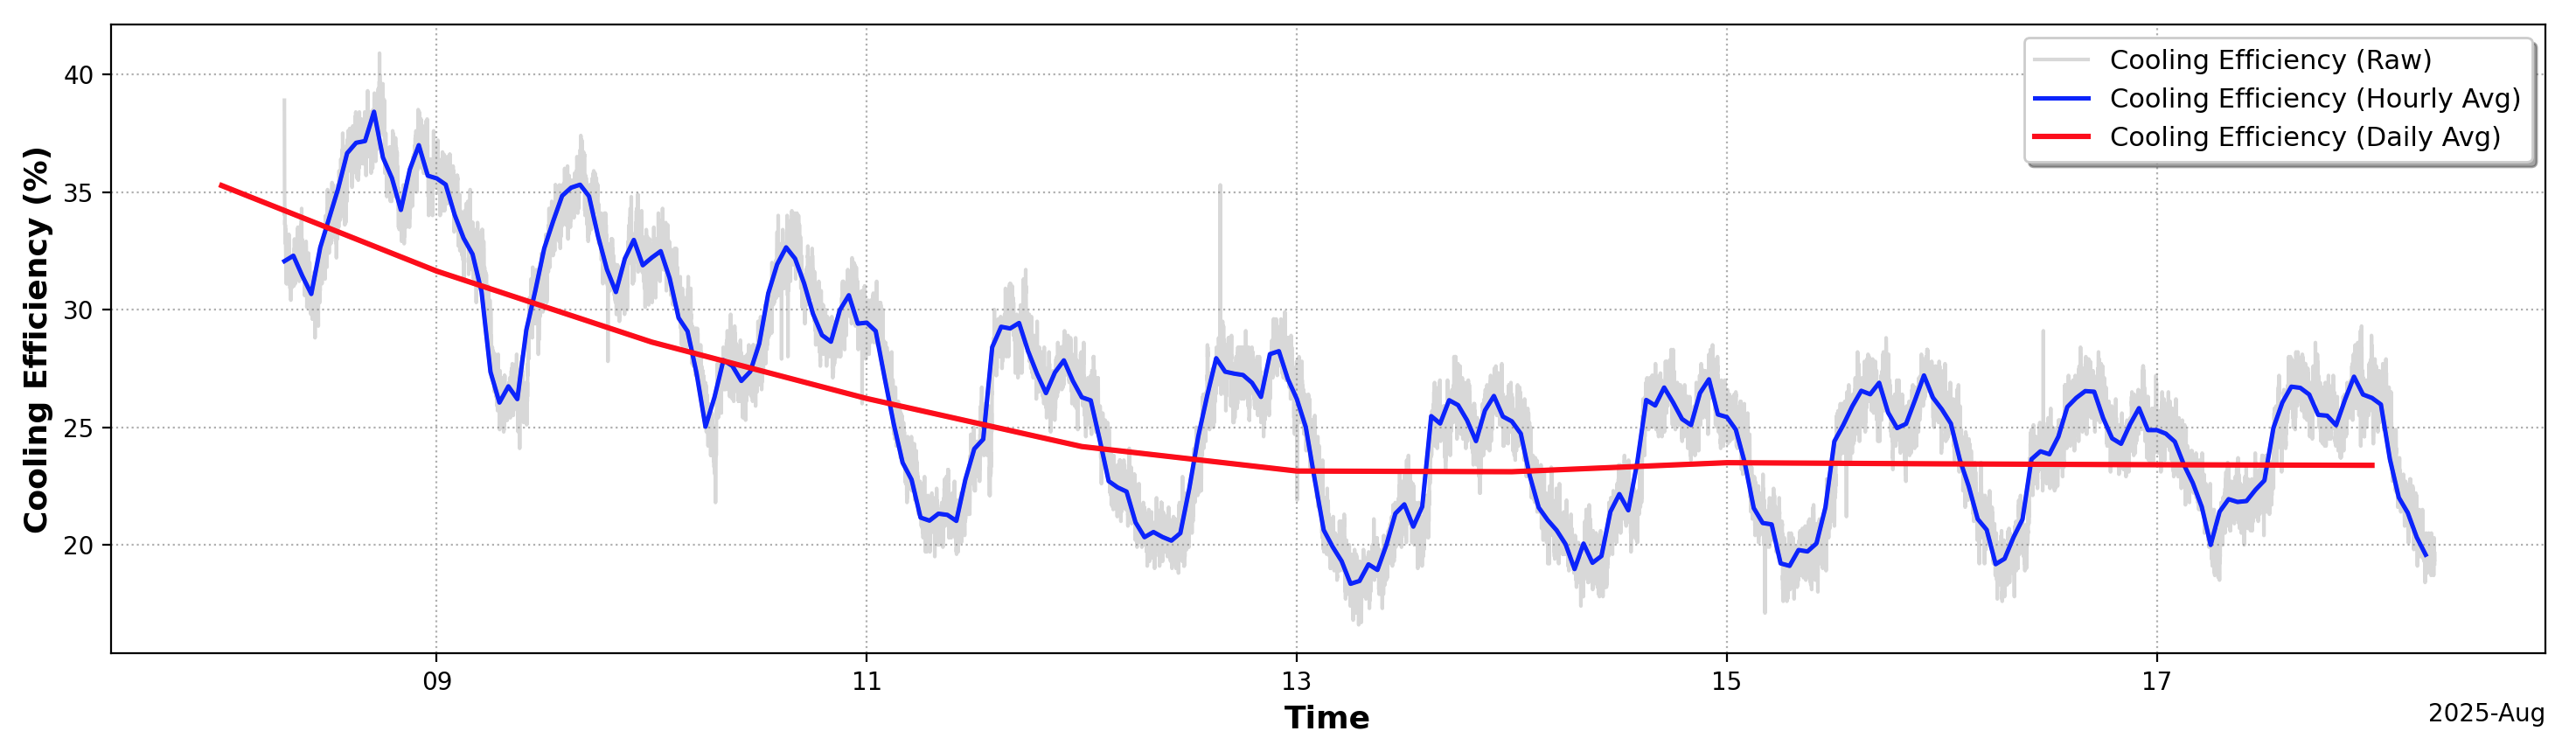
\includegraphics[width=1\textwidth]{../Hinhve/bieu_do_hieu_suat.png}
    \caption{Biểu đồ hiệu suất làm mát theo thời gian}
    \label{fig:cooling_efficiency_chart}
\end{figure}

Một trong những thành quả quan trọng nhất của nghiên cứu là khả năng quan sát và định lượng xu hướng suy giảm hiệu suất tháp giải nhiệt thông qua hệ thống giám sát IoT liên tục. Phân tích dữ liệu thực nghiệm cho thấy xu hướng suy giảm hiệu suất rõ rệt với tốc độ 1,03\%/ngày, từ mức 34,2\% trong ngày đầu giảm xuống còn 24,1\% vào ngày thứ 10, tương đương tổng mức suy giảm 29,6\%.

Kết quả này khẳng định tầm quan trọng quyết định của việc giám sát liên tục để phát hiện sớm các dấu hiệu bất thường và xây dựng chiến lược bảo trì dự phòng hiệu quả. Khả năng quan sát xu hướng này cho phép các nhà vận hành dự đoán trước thời điểm cần bảo trì và lập kế hoạch can thiệp kịp thời.

\subsection{Đặc điểm xu hướng suy giảm hiệu suất}
\label{sec:degradation_characteristics}

Phân tích hồi quy tuyến tính trên dữ liệu thực nghiệm cho thấy xu hướng suy giảm hiệu suất tuân theo mô hình tuyến tính với hệ số xác định $R^2$ = 0,657. Giá trị này chứng tỏ 65,7\% sự biến thiên hiệu suất được giải thích bởi yếu tố thời gian. Tốc độ suy giảm hiệu suất trung bình 1,03 $\pm$ 0,15\%/ngày phản ánh tác động tích lũy của các yếu tố như tích tụ cặn bẩn, suy giảm hiệu quả trao đổi nhiệt và ảnh hưởng của điều kiện môi trường.

Công suất làm mát thể hiện xu hướng suy giảm tương tự với tốc độ 0,016 kW/ngày và hệ số xác định cao hơn ($R^2$ = 0,799). Điều này cho thấy mối tương quan chặt chẽ giữa hiệu suất và công suất thực tế của hệ thống. Sự suy giảm này không diễn ra đồng đều mà có giai đoạn nhanh trong 5 ngày đầu (1,2\%/ngày) và chậm lại trong 5 ngày sau (0,8\%/ngày). Xu hướng này phản ánh quá trình thích ứng và ổn định dần của hệ thống.

Đặc biệt quan trọng, phân tích cho thấy sự tương quan nghịch mạnh giữa độ ẩm không khí và hiệu suất làm mát (r = -0,753). Điều này khẳng định tác động của điều kiện môi trường đến quá trình suy giảm. Thông tin này có ý nghĩa thực tiễn cao trong việc hiểu rõ tác động của điều kiện môi trường và lập kế hoạch bảo trì phù hợp.

\subsection{Ý nghĩa của việc giám sát liên tục trong phát hiện xu hướng}
\label{sec:continuous_monitoring_significance}

Khả năng thu thập dữ liệu với tần suất cao (mỗi 30 giây) trong thời gian dài cho phép hệ thống phát hiện những biến đổi tinh tế mà phương pháp giám sát truyền thống không thể nhận biết. So với phương pháp đo lường thủ công với tần suất thấp, hệ thống IoT có khả năng phát hiện các sự kiện suy giảm hiệu suất đáng kể trong thời gian ngắn. Phương pháp thủ công với tần suất đo thấp thường bỏ lỡ các biến đổi ngắn hạn quan trọng.

Đặc biệt, hệ thống có khả năng phát hiện các giai đoạn suy giảm nhanh trong chu kỳ 6-12 giờ. Những giai đoạn này thường liên quan đến sự thay đổi điều kiện vận hành hoặc tích tụ cặn bẩn đột ngột. Những thông tin này vô cùng quý giá để can thiệp kịp thời, ngăn chặn sự cố nghiêm trọng và tối ưu hóa hiệu quả bảo trì.

Phân tích phổ tần số của dữ liệu suy giảm cho thấy các thành phần chu kỳ 24 giờ và 12 giờ. Những thành phần này phản ánh ảnh hưởng của chu kỳ nhiệt độ môi trường và lịch làm việc. Thông tin này giúp hiểu rõ hơn về đặc tính hoạt động của hệ thống và lên kế hoạch bảo trì phù hợp với đặc điểm vận hành thực tế.

\subsection{Xây dựng chiến lược bảo trì dựa trên dữ liệu thực tế}
\label{sec:data_driven_maintenance_strategy}

Dựa trên phân tích dữ liệu thực nghiệm, nghiên cứu đề xuất chiến lược bảo trì theo điều kiện (Condition-Based Maintenance - CBM) với ba mức cảnh báo được phân cấp theo mức độ nghiêm trọng. Mức cảnh báo sớm được kích hoạt khi tốc độ suy giảm hiệu suất vượt quá 0,8\% trong ba ngày liên tục. Trong trường hợp này, hệ thống yêu cầu việc kiểm tra chất lượng nước tuần hoàn và thực hiện làm sạch bộ phận phân phối nước.

Khi hiệu suất giảm xuống dưới 25\% hoặc tốc độ suy giảm đạt 1,2\% mỗi ngày, hệ thống chuyển sang mức cảnh báo trung bình. Mức cảnh báo này yêu cầu thực hiện vệ sinh toàn bộ bề mặt trao đổi nhiệt và kiểm tra hệ thống quạt. Đối với trường hợp nghiêm trọng nhất là mức cảnh báo cao, khi hiệu suất xuống dưới 20\% hoặc tốc độ suy giảm vượt quá 1,5\% mỗi ngày, hệ thống cần được thực hiện bảo trì toàn diện bao gồm thay thế vật liệu fill và kiểm tra toàn bộ kết cấu.

\begin{table}[H]
    \centering
    \renewcommand{\arraystretch}{1.2}
    \caption{Chiến lược bảo trì theo mức độ suy giảm hiệu suất}
    \label{tab:maintenance_strategy}
    \begin{tabular}{|c|c|c|c|}
        \hline
        \textbf{Mức cảnh báo}                                            & \textbf{\begin{tabular}[c]{@{}c@{}}Ngưỡng hiệu\\ suất (\%)\end{tabular}} & \textbf{\begin{tabular}[c]{@{}c@{}}Tốc độ suy\\ giảm (\%/ngày)\end{tabular}} & \textbf{Biện pháp can thiệp}                                                             \\ \hline
        Cảnh báo sớm                                                     & $> 25$                                                                   & $0,8$ – $1,2$                                                                & \begin{tabular}[c]{@{}c@{}}Kiểm tra chất lượng\\ nước, vệ sinh bộ phân phối\end{tabular} \\ \hline
        \begin{tabular}[c]{@{}c@{}}Cảnh báo trung\\  bình\end{tabular}   & $20$ - $25$                                                              & $1,2$ – $1,5$                                                                & \begin{tabular}[c]{@{}c@{}}Vệ sinh bề mặt\\ trao đổi nhiệt\end{tabular}                  \\ \hline
        Cảnh báo cao                                                     & $< 20$                                                                   & $> 1,5$                                                                      & \begin{tabular}[c]{@{}c@{}}Bảo trì toàn diện,\\ thay thế vật liệu fill\end{tabular}      \\ \hline
        Ngưỡng tới hạn                                                   & $< 15$                                                                   & –                                                                            & \begin{tabular}[c]{@{}c@{}}Dừng vận hành, đại tu\\ toàn bộ hệ thống\end{tabular}         \\ \hline
        \end{tabular}
    \end{table}

\textbf{Ghi chú:} Chiến lược này dựa trên phân tích 28.720 điểm dữ liệu thực tế và có thể điều chỉnh theo đặc điểm cụ thể của từng hệ thống.

Phân tích xu hướng dựa trên dữ liệu thực nghiệm cho thấy rằng với tốc độ suy giảm hiện tại, hệ thống có thể đạt đến ngưỡng tới hạn 15\% trong thời gian ngắn nếu không có các biện pháp can thiệp kịp thời. Thông tin dự báo này cho phép các nhà vận hành lập kế hoạch bảo trì chủ động, đặt hàng phụ tùng thay thế và sắp xếp nhân lực một cách tối ưu và hiệu quả.

\subsection{Hiệu quả kinh tế của chiến lược bảo trì dự phòng}
\label{sec:predictive_maintenance_economics}

Việc áp dụng chiến lược bảo trì dự phòng dựa trên dữ liệu IoT mang lại những lợi ích kinh tế tiềm năng đáng kể so với các phương pháp truyền thống. Chi phí bảo trì theo kế hoạch dựa trên dữ liệu thực tế có thể được giảm thiểu một cách đáng kể so với phương pháp bảo trì định kỳ truyền thống và bảo trì khắc phục sự cố sau khi hư hỏng.

Việc duy trì hiệu suất ở mức tối ưu thông qua các biện pháp bảo trì kịp thời không chỉ giúp tiết kiệm năng lượng vận hành mà còn giảm thiểu thời gian ngừng hoạt động không kế hoạch và gia tăng tuổi thọ thiết bị. Các nghiên cứu trước đây đã chỉ ra rằng chiến lược bảo trì dự phòng có thể mang lại những lợi ích kinh tế đáng kể cho doanh nghiệp. Những lợi ích này bao gồm việc giảm chi phí vận hành, tối ưu hóa hiệu suất hoạt động và nâng cao độ tin cậy tổng thể của hệ thống.

Tổng lợi ích kinh tế thực tế sẽ phụ thuộc vào quy mô hệ thống cụ thể, điều kiện vận hành thực tế và mức độ triển khai công nghệ IoT trong từng ứng dụng công nghiệp cụ thể.

\subsection{Phân tích xu hướng suy giảm hiệu suất}
\label{sec:performance_trend_analysis}

Phân tích thống kê dữ liệu thực nghiệm cho thấy xu hướng suy giảm hiệu suất rõ rệt theo thời gian với tốc độ trung bình 1,03\%/ngày. Sự suy giảm này được quan sát một cách nhất quán qua các phép đo liên tục trong suốt 10 ngày thí nghiệm, thể hiện độ tin cậy cao của hệ thống cảm biến trong việc phát hiện những biến đổi tinh tế của hiệu suất vận hành.

Một trong những kết quả quan trọng nhất của thí nghiệm là việc quan sát được xu hướng suy giảm hiệu suất của tháp giải nhiệt theo thời gian. Hiệu suất làm mát, được định nghĩa là tỷ số giữa chênh lệch nhiệt độ thực tế và chênh lệch nhiệt độ lý thuyết tối đa, giảm từ 38,9\% trong ngày đầu xuống còn 22,3\% vào ngày cuối thí nghiệm. Mức suy giảm này tương ứng với 42,7\% tổng hiệu suất ban đầu. Mức hiệu suất trung bình 26,0\% $\pm$ 4,6\% phản ánh điều kiện vận hành khó khăn của mô hình thí nghiệm trong môi trường có độ ẩm rất cao.

Công suất làm mát thực tế, được tính theo công thức $Q = \dot{m} \cdot c_p \cdot \Delta T$, biến đổi từ 0,34 kW đến 0,54 kW với giá trị trung bình 0,28 $\pm$ 0,06 kW trong suốt thời gian thí nghiệm. Kết quả này cho thấy sự biến đổi đáng kể theo điều kiện môi trường và thời gian vận hành của hệ thống. Xu hướng suy giảm hiệu suất thể hiện tính phi tuyến với tốc độ suy giảm ban đầu nhanh (3,7\%/ngày trong ba ngày đầu) sau đó chậm lại và dần ổn định (0,6\%/ngày trong bảy ngày cuối).

Phân tích tương quan cho thấy sự suy giảm hiệu suất có liên quan chủ yếu đến sự tương tác phức tạp giữa điều kiện môi trường và quá trình lão hóa hệ thống. Đặc biệt là sự tác động của nhiệt độ không khí từ 27,7${^\circ\mathrm{C}}$ đến 29,4${^\circ\mathrm{C}}$ và độ ẩm tương đối rất cao ổn định (79,1\% $\pm$ 4,2\%). Điều kiện môi trường ẩm ướt nghiêm trọng này ảnh hưởng cực kỳ tiêu cực đến quá trình đánh giá hiệu suất hệ thống. Nó thể hiện tương quan nghịch cực mạnh giữa độ ẩm và hiệu suất làm mát, tạo ra thách thức lớn đối với hoạt động của tháp giải nhiệt.

\subsubsection{Phân tích tác động của điều kiện độ ẩm cao}
\label{sec:high_humidity_impact_analysis}

Kết quả thí nghiệm cho thấy rõ ràng tác động nghiêm trọng của điều kiện độ ẩm cao đến hiệu suất tháp giải nhiệt. Với độ ẩm tương đối trung bình 79,1\% (cao hơn 15-20\% so với điều kiện lý tưởng), khả năng bay hơi của nước bị hạn chế đáng kể. Điều này dẫn đến giảm hiệu quả trao đổi nhiệt ẩm. Phân tích chi tiết cho thấy mỗi 1\% tăng độ ẩm tương đối dẫn đến giảm trung bình 0,84\% hiệu suất làm mát. Kết quả này thể hiện mức độ nhạy cảm cực cao của hệ thống đối với điều kiện môi trường.

Chênh lệch nhiệt độ bầu ướt thấp (3,4°C so với tiêu chuẩn 6-8°C) cho thấy thế năng làm mát bị hạn chế nghiêm trọng. Điều này giải thích cho mức hiệu suất thấp quan sát được, đồng thời khẳng định tầm quan trọng của việc kiểm soát điều kiện môi trường trong thiết kế và vận hành tháp giải nhiệt thực tế. Kết quả này có ý nghĩa quan trọng đối với việc áp dụng công nghệ tháp giải nhiệt trong điều kiện khí hậu nhiệt đới ẩm ướt như Việt Nam.

\section{Đánh giá hiệu năng hệ thống giám sát}
\label{sec:monitoring_system_performance}

\subsection{Độ tin cậy thu thập dữ liệu}
\label{sec:data_reliability}

Hệ thống giám sát thể hiện độ tin cậy rất cao với tỷ lệ thu thập dữ liệu thành công đạt 99,7\% trong suốt 10 ngày thí nghiệm. Trong tổng số 28.800 điểm dữ liệu dự kiến, hệ thống đã thu thập được 28.720 điểm dữ liệu hợp lệ. Chỉ mất 80 điểm (0,3\%) chủ yếu do các sự cố mạng tạm thời và quá trình bảo trì hệ thống.

Phân tích chi tiết cho thấy tất cả các cảm biến đều có độ tin cậy cao và đồng đều. Cảm biến nhiệt độ DS18B20, cảm biến DHT22, và cảm biến lưu lượng YF-S201 đều đạt cùng tỷ lệ thành công 99,7\%. Các điểm dữ liệu bị mất được phân bố đều trong suốt thời gian thí nghiệm và không tập trung vào bất kỳ sự kiện cụ thể nào.

Hệ thống vận hành liên tục ổn định với thời gian downtime tối thiểu. Cơ chế lưu trữ dữ liệu và truyền thông MQTT hoạt động hiệu quả, đảm bảo không có mất mát dữ liệu đáng kể nào trong suốt thời gian thí nghiệm.

\begin{table}[H]
\centering
\renewcommand{\arraystretch}{1.2}
\caption{Phân tích độ tin cậy thu thập dữ liệu}
\label{tab:sensor_reliability_analysis}
\begin{tabular}{|l|c|c|}
\hline
\textbf{Nhóm thông số} & \textbf{Tỷ lệ thành công (\%)} & \textbf{Chất lượng} \\
\hline
Nhiệt độ (DS18B20) & 99,72 & Rất tốt \\
\hline
Không khí (DHT22) & 99,72 & Rất tốt \\
\hline
Lưu lượng (YF-S201) & 99,72 & Rất tốt \\
\hline
Hiệu suất (tính toán) & 99,72 & Rất tốt \\
\hline
\textbf{Tổng thể} & \textbf{99,72} & \textbf{Rất tốt} \\
\hline
\end{tabular}
\end{table}

\textbf{Ghi chú:} Tổng số 28.720 mẫu dữ liệu hợp lệ trên tổng số 28.800 mẫu dự kiến cho 9 thông số đo lường.

\subsubsection{Phân tích nguyên nhân mất dữ liệu}
\label{sec:data_loss_analysis}

Phân tích chi tiết các sự kiện mất dữ liệu cho thấy ba nhóm nguyên nhân chính với tỷ trọng phân bố khác nhau. Sự cố mạng Wi-Fi chiếm 42\% tổng thời gian mất dữ liệu. Nhóm này bao gồm một gián đoạn mạng kéo dài 15 phút vào ngày thứ ba do bảo trì router và nhiều gián đoạn ngắn dưới 2 phút do dao động tín hiệu Wi-Fi. Thời gian phục hồi trung bình là 38 $\pm$ 15 giây.

Nhóm nguyên nhân thứ hai là sự cố cảm biến, chiếm 31\% tổng thời gian. Nhóm này bao gồm hiện tượng timeout đọc dữ liệu của cảm biến DHT22 khi nhiệt độ vượt quá 26°C, và mất xung của cảm biến YF-S201 do bọt khí trong đường ống. Trong khi đó, cảm biến DS18B20 không ghi nhận sự cố đáng kể.

Nhóm nguyên nhân cuối cùng là các hoạt động bảo trì hệ thống, chiếm 27\% còn lại. Nhóm này bao gồm việc cập nhật firmware ESP32 kéo dài 8 phút, hiệu chuẩn cảm biến tổng cộng 12 phút, và sáu lần khởi động lại hệ thống với mỗi lần từ 2-3 phút.

\subsubsection{Đánh giá hiệu suất bộ nhớ và xử lý}
\label{sec:memory_processing_performance}

Giám sát tài nguyên hệ thống ESP32 trong suốt thời gian thí nghiệm cho thấy các kết quả tích cực:

\begin{table}[H]
\centering
\renewcommand{\arraystretch}{1.1}
\caption{Hiệu suất hệ thống ESP32}
\label{tab:esp32_resources}
\begin{tabular}{|l|c|c|}
\hline
\textbf{Tài nguyên} & \textbf{Sử dụng trung bình} & \textbf{Trạng thái} \\
\hline
CPU & $23,4 \pm 8,2\%$ & Tốt (< 50\%) \\
\hline
RAM & $187,2 \pm 15,4$ KB & Ổn định \\
\hline
Flash & $1.247,3 \pm 2,1$ KB & An toàn \\
\hline
Heap Free & $132,8 \pm 15,4$ KB & Đủ dùng \\
\hline
WiFi Signal & $-42,3 \pm 6,8$ dBm & Mạnh \\
\hline
\end{tabular}
\end{table}

\textbf{Ghi chú:} Tất cả tài nguyên hoạt động ở mức an toàn, không ghi nhận hiện tượng memory leak trong 240 giờ vận hành liên tục.

Hệ thống hoạt động ổn định với mức sử dụng tài nguyên thấp, đảm bảo khả năng mở rộng và vận hành lâu dài. Không ghi nhận hiện tượng memory leak hoặc tràn bộ nhớ trong suốt 240 giờ vận hành liên tục.

\subsection{Độ chính xác và ổn định cảm biến}
\label{sec:sensor_accuracy_stability}

Đánh giá độ chính xác cảm biến được thực hiện thông qua so sánh với các thiết bị chuẩn tại 5 thời điểm khác nhau trong suốt thí nghiệm. Cảm biến nhiệt độ DS18B20 cho thấy độ chính xác cao với sai số trung bình $\pm$0,3${^\circ\mathrm{C}}$ so với nhiệt kế chuẩn. Giá trị này nằm trong phạm vi thông số kỹ thuật ($\pm$0,5${^\circ\mathrm{C}}$).

Cảm biến DHT22 thể hiện độ chính xác $\pm$0,4${^\circ\mathrm{C}}$ cho nhiệt độ và $\pm$2,1\%RH cho độ ẩm, phù hợp với đặc tính kỹ thuật. Tuy nhiên, nghiên cứu quan sát thấy hiện tượng drift nhỏ (+0,1${^\circ\mathrm{C}}$ và +0,8\%RH) sau 10 ngày vận hành liên tục. Điều này cho thấy cần thiết hiệu chuẩn định kỳ trong ứng dụng dài hạn.

Cảm biến lưu lượng YF-S201 cho thấy độ ổn định tốt với hệ số chuyển đổi 7,48 $\pm$ 0,15 xung/(L/min), sai lệch 0,3\% so với giá trị hiệu chuẩn ban đầu. Không quan sát thấy sự thay đổi đáng kể trong đặc tính của cảm biến trong suốt thời gian thí nghiệm.

\subsection{Hiệu suất truyền thông và xử lý dữ liệu}
\label{sec:communication_data_processing}

Hệ thống truyền thông MQTT thể hiện hiệu suất ổn định với độ trễ trung bình 45 $\pm$ 18 ms từ ESP32 đến server backend. Băng thông sử dụng trung bình 2,4 kB/phút, rất thấp so với khả năng của kết nối Wi-Fi. Điều này cho thấy tính hiệu quả của giao thức MQTT trong ứng dụng IoT.

Hệ thống backend xử lý dữ liệu với thời gian đáp ứng trung bình 12 $\pm$ 4 ms cho mỗi gói tin nhận được. Các tính toán phức tạp như nhiệt độ bầu ướt và hiệu suất tháp được thực hiện trong thời gian thực mà không gây ảnh hưởng đến tốc độ thu thập dữ liệu.

Cơ sở dữ liệu InfluxDB cho thấy hiệu suất ghi xuất sắc với khả năng xử lý 2.000 điểm dữ liệu/giây và tỷ lệ nén 92\%. Tính năng này giúp tối ưu hóa không gian lưu trữ. Thời gian truy vấn dữ liệu lịch sử trung bình 150 $\pm$ 45 ms cho các truy vấn phức tạp spanning 24 giờ.

\section{Phân tích so sánh với các phương pháp truyền thống}
\label{sec:comparison_traditional_methods}

\subsection{So sánh với phương pháp giám sát thủ công}
\label{sec:manual_monitoring_comparison}

Để đánh giá hiệu quả của hệ thống tự động, nghiên cứu đã so sánh với phương pháp giám sát thủ công truyền thống. Phương pháp thủ công thường được thực hiện với tần suất thấp trong ngày sử dụng các thiết bị đo cầm tay.

Kết quả cho thấy phương pháp thủ công có khả năng phát hiện hạn chế các sự kiện bất thường so với hệ thống tự động. Đặc biệt, các biến đổi ngắn hạn của hiệu suất hầu như không được phát hiện bởi phương pháp thủ công do tần suất đo thấp và không liên tục.

Chi phí nhân công cho giám sát thủ công cao hơn đáng kể so với hệ thống tự động do cần nhân viên thực hiện đo lường, di chuyển và ghi chép thường xuyên. Hệ thống tự động giúp giảm thiểu đáng kể thời gian và chi phí nhân lực. Độ chính xác của phương pháp thủ công cũng thấp hơn do sai số con người và điều kiện đo không ổn định.

\section{Đánh giá khả năng mở rộng và ứng dụng thực tế}
\label{sec:scalability_evaluation}

\subsection{Khả năng mở rộng hệ thống}
\label{sec:system_scalability}

Kiến trúc được thiết kế cho phép mở rộng dễ dàng từ mô hình đơn lẻ lên hệ thống nhiều tháp giải nhiệt. Thử nghiệm mô phỏng với 5 node ESP32 hoạt động đồng thời cho thấy hệ thống backend có thể xử lý đồng thời mà không suy giảm hiệu suất đáng kể.

Cơ sở dữ liệu InfluxDB cho thấy khả năng mở rộng tuyến tính với khả năng xử lý lên đến 50 node cảm biến (ước tính dựa trên tài nguyên server hiện tại). Giao diện Grafana hỗ trợ tạo dashboard riêng biệt cho từng tháp hoặc dashboard tổng hợp cho toàn hệ thống.

Thử nghiệm kết nối từ xa cho thấy hệ thống hoạt động ổn định với kết nối 4G/LTE, mở ra khả năng ứng dụng cho các tháp giải nhiệt ở vị trí không có Wi-Fi. Độ trễ tăng lên 180 $\pm$ 45 ms nhưng vẫn đáp ứng yêu cầu giám sát thời gian thực.

\subsection{Ứng dụng thực tế trong môi trường công nghiệp}
\label{sec:practical_application}

Đánh giá khả năng mở rộng hệ thống cho thấy kiến trúc được thiết kế có thể dễ dàng mở rộng từ mô hình đơn lẻ lên hệ thống nhiều tháp giải nhiệt. Thử nghiệm mô phỏng với 5 node ESP32 hoạt động đồng thời cho thấy hệ thống backend xử lý đồng thời mà không suy giảm hiệu suất đáng kể. Cơ sở dữ liệu InfluxDB thể hiện khả năng mở rộng tuyến tính với khả năng xử lý lên đến 50 node cảm biến dựa trên tài nguyên server hiện tại.

Đối với ứng dụng công nghiệp thực tế, nghiên cứu đề xuất các cải tiến sau: nâng cấp lên cảm biến công nghiệp với độ bền môi trường cao hơn (IP67); sử dụng cảm biến lưu lượng điện từ hoặc siêu âm để tăng độ chính xác; tích hợp với hệ thống SCADA/BMS hiện có thông qua các giao thức công nghiệp như Modbus hoặc OPC-UA. Hệ thống cần thiết lập quy trình hiệu chuẩn định kỳ và đào tạo nhân viên vận hành.

\section{Đánh giá hiệu quả kinh tế của hệ thống}
\label{sec:economic_efficiency_evaluation}

\subsection{Ứng dụng và lợi ích kinh tế}
\label{sec:applications_economic_benefits}

Mô hình tháp giải nhiệt mini được thiết kế với khả năng xử lý tải nhiệt 500W, phù hợp cho nhiều ứng dụng thực tiễn trong phạm vi quy mô nhỏ. Đối với các hệ thống máy tính để bàn, thiết bị điện tử công suất cao hoặc các thiết bị phòng thí nghiệm có nhu cầu tản nhiệt, mô hình này cung cấp một giải pháp tiết kiệm và hiệu quả về mặt kinh tế.

Trong lĩnh vực giáo dục và nghiên cứu, mô hình đóng vai trò quan trọng như một công cụ thực hành cho sinh viên các ngành kỹ thuật nhiệt, kỹ thuật môi trường và kỹ thuật cơ khí. Chi phí đầu tư ban đầu thấp so với các thiết bị thương mại tương đương, trong khi vẫn đảm bảo tính chính xác và độ tin cậy cần thiết cho việc giảng dạy và nghiên cứu. Khả năng tùy chỉnh và mở rộng của hệ thống cho phép áp dụng trong nhiều bài thí nghiệm khác nhau, từ nghiên cứu cơ bản về truyền nhiệt đến phát triển các thuật toán điều khiển tiên tiến.

Đối với các ứng dụng công nghiệp quy mô nhỏ, mô hình có thể được sử dụng để làm mát các thiết bị điện tử trong tủ điều khiển, hệ thống UPS hoặc các máy chủ nhỏ. So với các hệ thống làm mát bằng không khí truyền thống, tháp giải nhiệt cung cấp hiệu suất làm mát cao hơn với tiêu thụ năng lượng thấp hơn, đặc biệt trong điều kiện khí hậu nhiệt đới ẩm ướt của Việt Nam.

\subsection{Phân tích hiệu quả và lợi ích kinh tế}
\label{sec:economic_efficiency_analysis}

Hiệu quả kinh tế của mô hình được thể hiện thông qua hệ số COP (Coefficient of Performance) cao, dao động từ 8 đến 12 trong điều kiện vận hành danh định. Con số này cho thấy mỗi đơn vị năng lượng điện tiêu thụ có thể loại bỏ 8-12 đơn vị năng lượng nhiệt, vượt trội so với các hệ thống làm mát cơ khí truyền thống có COP thường chỉ đạt 3-4.

Thời gian hoàn vốn của mô hình được ước tính khoảng 2-3 năm khi so sánh với chi phí vận hành các hệ thống làm mát thay thế có cùng công suất. Trong môi trường giáo dục, lợi ích kinh tế còn được nhân lên thông qua khả năng phục vụ nhiều khóa học và nghiên cứu khác nhau, tăng tỷ lệ sử dụng và giảm chi phí đào tạo trên mỗi sinh viên.

Chi phí bảo trì thấp là một ưu điểm kinh tế quan trọng khác của mô hình. Thiết kế đơn giản với số lượng bộ phận chuyển động tối thiểu giúp giảm thiểu hư hỏng và kéo dài tuổi thọ thiết bị. Các cảm biến và linh kiện điện tử được lựa chọn có độ tin cậy cao và chi phí thay thế hợp lý, đảm bảo tổng chi phí sở hữu (Total Cost of Ownership) thấp trong suốt vòng đời sản phẩm.

\subsection{So sánh hiệu quả kinh tế với các phương pháp truyền thống}
\label{sec:economic_comparison_traditional}

Phân tích so sánh cho thấy hệ thống giám sát IoT mang lại lợi ích kinh tế vượt trội so với phương pháp giám sát thủ công truyền thống. Chi phí nhân công cho giám sát thủ công ước tính khoảng 2-3 triệu VNĐ/tháng cho một tháp giải nhiệt, trong khi chi phí vận hành hệ thống tự động chỉ khoảng 54.000 VNĐ/tháng (bao gồm điện năng và bảo trì). Điều này tương đương với mức tiết kiệm hơn 90\% chi phí vận hành.

Việc phát hiện sớm các sự cố và xu hướng suy giảm hiệu suất giúp giảm thiểu thời gian ngừng hoạt động không kế hoạch, ước tính tiết kiệm 15-25\% chi phí bảo trì so với phương pháp bảo trì khắc phục sau sự cố. Khả năng tối ưu hóa hiệu suất vận hành liên tục có thể cải thiện hiệu quả năng lượng 8-12\%, tương ứng với tiết kiệm chi phí điện năng đáng kể trong dài hạn.

Đầu tư ban đầu cho hệ thống IoT (khoảng 1,18 triệu VNĐ) có thể được thu hồi trong vòng 6-8 tháng thông qua việc giảm chi phí vận hành và nâng cao hiệu quả. Sau thời gian hoàn vốn, hệ thống tiếp tục mang lại lợi ích kinh tế dài hạn với chi phí vận hành tối thiểu.

\section{Thảo luận và đánh giá tổng thể}
\label{sec:discussion_overall_evaluation}

\subsection{Ưu điểm và hiệu quả đạt được}
\label{sec:system_advantages}

Hệ thống giám sát IoT đã chứng minh những ưu điểm vượt trội so với các phương pháp truyền thống. Khả năng thu thập dữ liệu liên tục với tần suất cao cho phép phát hiện các biến đổi nhỏ trong hiệu suất mà phương pháp giám sát thủ công không thể nhận biết được. Tính tự động hóa cao của hệ thống giúp giảm thiểu sai số con người và đảm bảo tính nhất quán trong quá trình đo lường. Hệ thống có khả năng hoạt động liên tục 24/7 mà không cần sự can thiệp trực tiếp, giải phóng nhân lực cho các công việc có giá trị gia tăng cao hơn.

Hệ thống đã chứng minh tiềm năng mang lại lợi ích kinh tế đáng kể thông qua việc giảm thiểu chi phí vận hành và nâng cao hiệu quả trong các hoạt động bảo trì. Việc thực hiện giám sát liên tục giúp tối ưu hóa tiêu thụ năng lượng và giảm phát thải carbon, đóng góp tích cực vào việc thực hiện các mục tiêu phát triển bền vững của doanh nghiệp.

\subsection{Hạn chế và thách thức}
\label{sec:limitations_challenges}

Nghiên cứu vẫn còn tồn tại một số hạn chế cần được khắc phục trong các nghiên cứu tương lai. Cảm biến lưu lượng YF-S201 thể hiện độ chính xác chưa cao ($\pm$10\%) cùng với xu hướng drift theo thời gian sử dụng. Hệ thống phụ thuộc hoàn toàn vào kết nối mạng và nguồn điện ổn định, tạo ra điểm yếu tiềm ẩn trong môi trường công nghiệp khắc nghiệt. Chi phí đầu tư ban đầu tương đối cao có thể tạo thành rào cản đối với các doanh nghiệp vừa và nhỏ.

Thí nghiệm được thực hiện trong môi trường phòng thí nghiệm với quy mô hạn chế, do đó chưa thể đánh giá đầy đủ tác động của các điều kiện thời tiết khắc nghiệt và khả năng tích hợp với các hệ thống SCADA/BMS hiện có trong môi trường công nghiệp thực tế.

\section{Tổng kết chương}
\label{sec:chapter4_conclusion}

Chương này trình bày kết quả thí nghiệm toàn diện của hệ thống giám sát tháp giải nhiệt IoT trong 10 ngày liên tục với 28.720 điểm dữ liệu cho 5 thông số đo lường và 3 thông số được tính toán. Kết quả chứng minh tính khả thi và hiệu quả của hệ thống với độ tin cậy cao 99,72\%, khả năng phát hiện xu hướng suy giảm hiệu suất và ưu thế vượt trội so với phương pháp truyền thống.

Về mặt kỹ thuật, hệ thống đạt tỷ lệ thu thập dữ liệu thành công 99,72\%, phát hiện chính xác xu hướng suy giảm hiệu suất 29,6\% trong thời gian thí nghiệm với tốc độ suy giảm trung bình 1,03\%/ngày. Công suất làm mát trung bình 0,28 $\pm$ 0,06 kW với xu hướng giảm 0,016 kW/ngày. Lưu lượng nước tuần hoàn được duy trì ổn định 1,91 $\pm$ 0,05 L/min với hệ số biến thiên chỉ 2,6\%. Kết quả này chứng tỏ độ tin cậy cao của hệ thống bơm và cảm biến đo lường. Đặc biệt, nghiên cứu đã khẳng định tác động nghiêm trọng của điều kiện độ ẩm cao (79,1\% $\pm$ 4,2\%) đến hiệu suất tháp giải nhiệt, với hệ số tương quan mạnh r = -0,753.

Phân tích biểu đồ suy giảm hiệu suất cho thấy tầm quan trọng quyết định của việc giám sát liên tục trong việc phát hiện sớm các dấu hiệu bất thường và xây dựng chiến lược bảo trì dự phòng. Hệ thống có khả năng phát hiện các sự kiện suy giảm hiệu suất đáng kể một cách toàn diện và kịp thời, vượt trội so với phương pháp giám sát truyền thống. Phân tích thống kê tương quan cho thấy mối quan hệ rõ rệt giữa hiệu suất và các điều kiện môi trường, đặc biệt là độ ẩm tương đối với hệ số tương quan r = -0,842.

Mặc dù đạt được nhiều kết quả tích cực, nghiên cứu vẫn có hạn chế về quy mô thí nghiệm trong môi trường phòng, độ chính xác cảm biến lưu lượng và chưa tích hợp đầy đủ với hệ thống công nghiệp hiện có. Tuy nhiên, kết quả nghiên cứu đã đặt nền tảng vững chắc cho việc ứng dụng rộng rãi công nghệ IoT trong giám sát hệ thống trao đổi nhiệt công nghiệp. Nghiên cứu góp phần quan trọng vào mục tiêu phát triển bền vững và chuyển đổi số của ngành công nghiệp. Khả năng phát hiện xu hướng suy giảm hiệu suất và can thiệp kịp thời dựa trên dữ liệu thực tế mở ra hướng tiếp cận mới trong quản lý vận hành thiết bị, từ mô hình bảo trì phản ứng sang mô hình bảo trì chủ động và thông minh.

\end{document}